\begin{frame}
\frametitle{Render Pass}
\begin{columns}

\column{.4\textwidth}

\begin{itemize}
\item Durante la fase di setup creiamo un render pass
\item Un render pass ci permette di descrivere le immagini (attachment) che vengono utilizzate durante il rendering
\item Un render pass suddivide le operazioni di rendering che utilizzano le stesse immagini in uno o più subpass
\end{itemize}

\column{.4\textwidth}

\begin{figure}[ht]
    \centering
    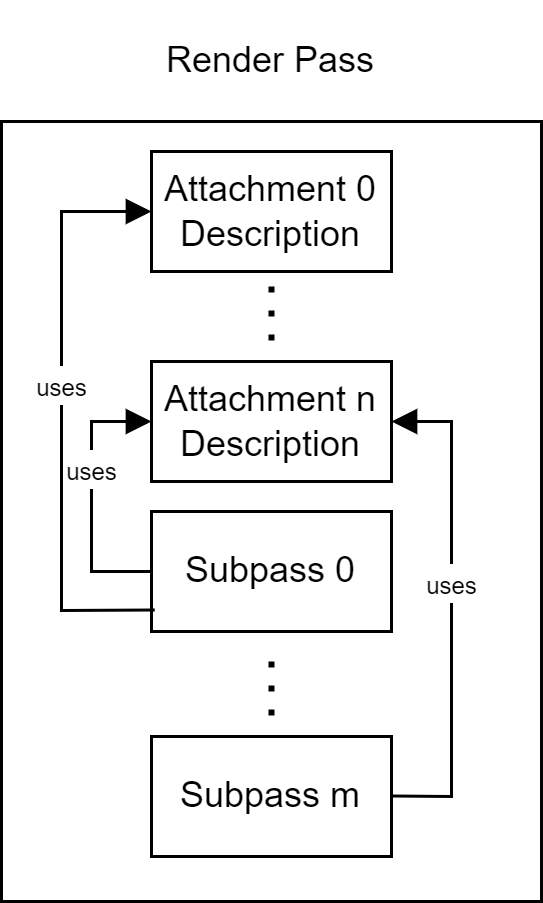
\includegraphics[scale=0.2]{images/SlidesClearWindow/RenderPass.png}
\end{figure}

\end{columns}
\end{frame}
